\chapter{实验}
\section{算法实现}
本文先使用OpenCV~\footnote{\url{https://opencv.org}}来对视频进行按照每0.5秒提取一张帧图像并保存到存储设备里,而提取帧图像的深度卷积特征是基于MxNet框架~\footnote{\url{http://mxnet.incubator.apache.org}},具体提取特征的代码项目video-cnn-feat~\footnote{\url{https://github.com/xuchaoxi/video-cnn-feat}}已经在github上开源。本文使用的两个预训练卷积神经网络(ResNet-152和ResNeXt-101)对实验数据提取的视觉特征~\footnote{\url{https://github.com/li-xirong/avs}}也已经在github上发布,每个视频的两种视觉特征都是2048维,而两种特征的拼接后的特征是4096维,每个视频的特征是由帧图像的特征进行平均池化操作得到的。

本文的W2VV++算法模型和SEA算法模型均使用PyTorch~\cite{pytorch}的深度学习框架实现,使用基于随机梯度下降法的RMSProp优化器对模型进行训练,优化器的学习率
根据实验经验设为0.0001,而其他参数使用默认值。为了防止训练时出现梯度爆炸,本研究把训练时的梯度降低L2范数倍。学习率在每次训练结束
后降为原来的0.99倍,如果模型在验证集上的性能连续三次没有提高则学习率降为原来的0.5倍。如果在验证集的性能连续10次没有提高,则模型训练
提前停止。本文最后测试的模型是在验证集上性能最好的模型。

模型训练的每个批次的大小为128对相关的句子-视频对,在每个批次给定的一个句子,本文把该批次里的其余剩余视频当作该句子的不相关视频,
即该句子与这些不相关视频构成负样本,而本文使用的最难负例来计算损失的策略,即选择这些负例中的最不相关的句子视频对来最后计算损失,
具体是余弦相似度最大的句子视频对作为最难负例。本文的W2VV++模型和SEA模型所有的公共跨模态空间的维度设为2048维。根据Faghri等人的文献~\cite{faghri2017vse++},目标函数公式\ref{eq:itrl}的超参数$\alpha$设为0.2。为了避免出现过拟合,本文在转换网络的全连接层使用概率为0.2的随机失活策略。本文的所有实验都在具有Nvidia GEFORCE GTX 1080Ti GPU显卡的服务器上进行。

\section{实验设置}
为了验证本文提出的W2VV++模型和SEA模型的有效性,本文在两个公开的视频数据基准线:MSR-VTT~\cite{msrvtt}和TRECVID AVS~\cite{awad2016trecvid}上进行实验。尽管MSR-VTT最初是用来研究视频描述生成的数据集,但是也有很多的基于文本的视频检索的工作~\cite{mithun2018learning,miech2019howto100m,dong2019dual,liu2019use,yu2018a}在该数据集上进行了尝试,TRECVID AVS是自从2016年以来在即席视频检索领域一个大规模的非常重要的基准线~\cite{awad2016trecvid,awad2017trecvid,awad2018trecvid,awad2019trecvid},这两个基准线都有各自的特点。如表格~\ref{tab:datasets}所示,MSR-VTT的测试数据集的视频数量相对较少,只有2,990个视频,而每个视频具有20个句子描述,一共59,800个句子描述。而TRECVID AVS具有大量的测试视频,在2016、2017和2018年的测试里面有超过了33.5万个测试视频,在2019年有超过100万个测试视频。因此,在这两个数据基准线上进行详尽的实验可以公平地验证算法模型的有效性。

\begin{table} [tb!]
\renewcommand{\arraystretch}{1.2}
    \caption[本文实验所用的数据集]{\textbf{本文实验所用的数据集}。 本文所有的实验均用对应的训练集(train set)对模型进行训练,用对应的验证集(val. set)对模型进行验证,用对应的测试集(test set)对模型进行测试。}

\label{tab:datasets}
\centering
 \scalebox{0.87}{
 \begin{tabular}{@{} |l | l |r |r|r|r|r|@{}}
\hline


     \textbf{数据划分} & \textbf{数据名称} & \textbf{视频数} & \textbf{帧数} & \textbf{查询数} & \textbf{bow词典} & \textbf{GRU词典} \\
\hline
\multicolumn{7}{|l|}{\textbf{MSR-VTT 实验:}} \\
\hline
     \textit{train set} & \multirow{4}{*}{MSR-VTT~\cite{msrvtt}} & 6,513 & 197,648 & -- & 7,676 & 7,807 \\
\cline{1-1}  \cline{3-7} 
     \textit{val. set} &  & 497 & 15,347 & 9,940 & -- & -- \\
\cline{1-1}  \cline{3-7}
     \textit{test-full} &  & 2,990 & 92,467 & 59,800 & -- & -- \\
\cline{1-1}  \cline{3-7}
     \textit{test-1k}~\cite{yu2018a} &  & 1,000 & 30,932 & 1,000 & -- & -- \\

\hline
\hline
\multicolumn{7}{|l|}{\textbf{TRECVID 实验:}} \\
\hline
     \multirow{2}{*}{\textit{train set}} & MSR-VTT~\cite{msrvtt}  & 10,000 & 305,462 & --  & \multirow{2}{*}{11,147} & \multirow{2}{*}{11,282} \\
\cline{2-5}
     & TGIF~\cite{li2016tgif}   & 100,855 & 1,045,268 & -- &  & \\
\hline
     \textit{val. set} & TV16-VTT-dev~\cite{awad2016trecvid}  & 200 & 5,941 & 200  & -- & -- \\
\hline
     \specialcell{\textit{test set} for \\ TV16/17/18} & IACC.3~\cite{awad2016trecvid}  & 335,944 & 3,845,221 & 90 & -- & -- \\
\hline
     \specialcell{\textit{test set} for \\TV19} & V3C1~\cite{berns2019v3c1} & 1,082,649 & 7,839,450 & 30 & -- & -- \\
\hline
\end{tabular}
 }% end of scalebox
\end{table}


%\begin{table} [tbh!]
%    \caption[AVS数据集]{这是AVS数据集的基本统计描述}
%    \label{tab:avs-dataset}
%    \centering
%    \scalebox{0.96}{
%        \begin{tabular}{@{}l r r r r r@{}}
%            \toprule
%            \textbf{数据集名称} & \textbf{镜头数} & \textbf{帧数} & \textbf{句子数} & \textbf{bow词典大小} & \textbf{GRU词典大小} \\
%            \hline
%            \emph{训练集:} & & & & & \\
%            MSR-VTT & 10,000 & 305,462 & 200,000 & \multirow{2}{*}{11,147} & \multirow{2}{*}{11,282} \\
%            TGIF & 100,855 & 1,045,268 & 124,534 & & \\
%            \hline
%            \emph{验证集:} & & & & & \\ 
%            TV16-VTT-train & 200 & 5,941 & 200 & - & - \\
%            \hline
%            \emph{测试集:} & & & & & \\
%            IACC.3 & 335,944 & 3,845,221 & - & - & - \\
%            V3C1 & 1,082,649 & 7,839,450 & - & - & - \\
%            \bottomrule
%        \end{tabular}
%    }
%\end{table}



\subsection{MSR-VTT 实验设置} \label{ssec:setup-msrvtt}
\textbf{数据划分}:本文根据MSR-VTT数据官方的数据划分,共分为三个没有交集的子集作为训练集、验证集和测试集,其中训练数据包含6,513个视频,130,260个句子描述,而验证集包含497个视频,9,940个句子描述作为查询,测试集包含2,990个视频,59,800个句子描述作为查询。而在文献~\cite{liu2019use,miech2019howto100m,yu2018a}中,这些工作在原来的测试集里随机采样了1,000个视频作为一个更小的测试集,而查询句子也进行了随机采样得到1,000个句子,每个视频对应一个句子描述。本文为了与这些工作进行公平的比较,也使用了这个更小的测试集,命名为\textit{test-1k},而原来的完整测试集命名为\textit{test-full}。

\textbf{性能指标}:根据之前的工作~\cite{dong2019dual,mithun2018learning},本文在MSR-VTT实验报告的指标为R@k, k=1,5,10,表示测试查询样例在前k个查询结果中至少有一个相关视频的百分比,该值越大模型效果越好,排序中位数(Median rank, Med r),表示在查询结果中第一个相关视频的排序的中位数,该值越小模型效果越好,和平均精度均值(Mean Average Precision, mAP)作为模型整体性能的指标,在验证集上也是使用mAP作为选择最优模型的指标。

\subsection{TRECVID 实验设置} \label{ssec:setup-tv}

\textbf{训练集}:如表格~\ref{tab:datasets}所示,本文的TRECVID实验使用MSR-VTT~\cite{msrvtt}和TGIF~\cite{li2016tgif}两个数据结合作为训练集。MSR-VTT数据包含1万个网络视频片段和20万个描述视频片段内容的句子,即每个视频片段有20个描述句子。
本文每段MSR-VTT的视频每半秒提取一帧的频率进行均匀采样,共生成305,462张帧图像。而TGIF数据包含超过10万张动图和12万个描述动图内容的句子,本文同样对每个动图进行均匀采样,共生成1,045,268张帧图像。

\textbf{验证集}:本文使用TRECVID 2016 Video-to-Text任务~\cite{awad2016trecvid}的训练集作为验证集,命名为TV16-VTT-dev,用于模型训练阶段的对最优模型的选择。这个集合共包含200个视频,每个视频含有2个描述视频内容的句子。对于每个视频,本文选择第一个句子作为该视频的文本查询,
而剩余的199个视频则是该查询的不相关视频。相应地,本文使用平均精度均值(mAP)作为评价模型在该验证集以文本检索视频的性能指标。

\textbf{视频测试集}:本文使用TRECVID的AVS任务在2016年至2018年使用的官方测试视频集IACC.3~\cite{awad2016trecvid}和在2019年使用的官方测试视频集V3C1~\cite{berns2019v3c1}。IACC.3数据集包含4,953个网络视频(600小时),视频的时长从6.5分钟到9.5分钟,平均时长为7.8分钟。
官方已经对视频做了自动镜头边界检测,共生成335,944个视频片段,用户的检索目标是这些独立的视频片段。本文同样对每个视频片段进行均匀采样,共生成3,845,221张帧图像。而TRECVID AVS 2019年使用的V3C1视频集是一个更大的未被标注的视频数据集,共包含了7,475个网络视频(1000小时),平均每个视频长为8分钟,同样,TRECVID官方对视频做了镜头自动分割,共被划分为1,082,649个视频片段。本文使用均匀采样对这些视频片段提取帧图像,共生成7,839,450张帧图像。

\textbf{查询测试集}:TRECVID的AVS任务每年定义30个查询来进行测试,每个查询是自然语言的句子形式,具有不同的长度和不同的语义难度。
例如“Find shots of palm trees”,“Find shots of a man with beard and wearing white robe speaking and gesturing to camera”和
“Find shots of a truck standing still while a person is walking beside or in front of it”。所有的查询均以“Find shots of”的短语开头,因此在测试时可以很容易地去掉而关注查询的主体部分。

\textbf{性能指标}:本文使用TRECVID AVS任务的官方评测指标,推测平均准确率(inferred average precision, infAP)~\cite{awad2016trecvid,awad2017trecvid,awad2018trecvid,awad2019trecvid}作为模型的评价指标,而模型的总体性能是所有测试查询样例的infAP分数的平均值,该值越高,模型的视频检索效果越好,本文以2016-2019年的infAP的平均值(AVG)作为模型在TRECVID上的整体性能。


\section{实验结果}
本文从消融实验和与先进方法的比较实验两个方面验证本文提出的W2VV++模型和SEA模型的有效性,消融实验可以验证不同模块对于模型的作用,从而验证本文提出的对于特定模块的改进的有效性,与目前的先进方法进行比较实验可以验证本文所提出的算法模型在即席视频检索领域具有优越性。

\subsection{消融实验}
\textbf{视频特征的选择}:本文比较了三种特征的选择,即$ResNeXt$,$ResNet$和$ResNeXt$-$ResNet$,分别表示ResNeXt-101特征,ResNet-152特征和这两个特征的拼接组成的特征。如表格~\ref{tab:tee_vs_w2vvpp}所示,对于模型W2VV++和SEA,使用ResNeXt-101的视频的特征比使用ResNet-152的效果好,而使用这两个特征拼接组成的$ResNeXt$-$ResNet$视频特征可以进一步提高这两个模型的性能。对于相同的视频特征,本文提出的W2VV++模型和SEA模型都比基础模型W2VV的效果好,其中SEA模型的效果最好。本文接下来的实验均以拼接的特征$ResNeXt$-$ResNet$进行实验,除非特别说明。



\begin{table*}[tbh!]
\normalsize
\renewcommand\arraystretch{1.2}
\centering
\caption{\textbf{Joint evaluation of sentence encoders and their assembly models, \ie W2VV++ and the proposed \emph{SEA}, on MSR-VTT and TRECVID}. Numbers are shown in percentages, with top performers highlighted in \best{bold} font. For a given setup of sentence encoders, relative improvement of SEA over its W2VV++ counterpart is given in parentheses, showing that SEA is consistently better.}
\label{tab:tee_vs_w2vvpp}
\scalebox{0.75}{
\begin{tabular}{@{}|l | l | r | r | r | r | l|| r | r | r | r | l|@{}}
\hline
\multirow{2}{*}{\textbf{模型}} & \multirow{2}{*}{\textbf{视频特征}} & \multicolumn{5}{c||}{\textbf{MSR-VTT} (test-full)} & \multicolumn{5}{c|}{\textbf{TRECVID} (指标: infAP)}  \\
\cline{3-12}
 & & \textit{R@1} & \textit{R@5} & \textit{R@10} & \textit{Med r} & \textit{mAP} & \textit{TV16} & \textit{TV17} & \textit{TV18} & \textit{TV19} & \textit{AVG}  \\

\hline
\multirow{3}{*}{W2VV++} & $ResNet$ &  &  &  &  & & & & & & \\

\cline{2-12}
 & $ResNeXt$ &  & & & & & 14.0 & 17.1 & 10.3 & & \\

\cline{2-12}   
 & $ResNeXt$-$ResNet$ & 11.1 & 29.6 & 40.5 & 18 & 20.6  & 16.2 & 22.3 & 10.1 & 13.9 & 15.6 \\

\hline
\multirow{3}{*}{SEA} & $ResNet$ & & & & & & & & & & \\

\cline{2-12}
 & $ResNeXt$ & & & & & & & & & & \\

\cline{2-12}
    & $ResNeXt$-$ResNet$ & \best{12.2} & \best{31.9} & \best{43.1} & \best{15} & \best{22.1} & 15.0 & \best{23.4} & \best{12.2} & \best{16.6} & \best{16.8} \\

\hline 

\end{tabular}
}
\end{table*}


\textbf{目标函数}:本文提出的W2VV++模型在W2VV模型的基础上对目标函数和GRU编码器的使用做了改进,即使用ITRL目标函数替换原来的均方误差(MSE)目标函数,使用GRU输出的所有隐藏层状态的平均替换原来的只取GRU输出的最后时刻的隐藏层状态。如表格~\ref{tab:loss_fusion}前三行所示,W2VV$_{ITRL}$表示在模型W2VV的基础上只将ITRL替换MSE,由结果可以看出,使用ITRL目标函数可以大幅提高基于文本的视频检索模型的性能,而本文提出的W2VV++可以进一步提高视频检索的效果。对于SEA的目标函数选择,本文已经在图~\ref{fig:negative-examples}定性地分析了多目标函数(combined loss)融合文本编码器的比单目标函数(single loss)的方式更好,本文通过实验进一步验证了这个结论。如表格~\ref{tab:loss_fusion}的最后两行显示,在两个数据集上,多目标函数的方式都比单目标函数的方式的效果好。



\begin{table*}[tbh!]
\normalsize
\renewcommand\arraystretch{1.2}
\centering
    \caption[在MSR-VTT和TRECVID上联合评测目标函数不同的模型和文本编码器融合方式不同的模型]{\textbf{在MSR-VTT和TRECVID上联合评测目标函数不同的模型和文本编码器融合方式不同的模型}。评价指标除了中位排序数Med r均以百分数的形式显示(\%),其中最好的结果用\best{粗体}标出。本文提出的W2VV++模型对基础模型W2VV的目标函数的改进起到了很大的作用,并且也更有效地使用了GRU编码器,而使用多空间多目标函数融合文本编码器的SEA模型的性能最好。}
\label{tab:loss_fusion}
\scalebox{0.79}{
\begin{tabular}{@{}|l | r | r | r | r | l|| r | r | r | r | l|@{}}
\hline
\multirow{2}{*}{\textbf{模型}} & \multicolumn{5}{c||}{\textbf{MSR-VTT} (test-full)} & \multicolumn{5}{c|}{\textbf{TRECVID} (指标: infAP)}  \\
\cline{2-11}
 & \textit{R@1} & \textit{R@5} & \textit{R@10} & \textit{Med r} & \textit{mAP} & \textit{TV16} & \textit{TV17} & \textit{TV18} & \textit{TV19} & \textit{AVG}  \\

\hline
W2VV & 1.1 & 4.7 & 8.0 & 240 & \textcolor{white}{0}3.7 & 1.3 & 0.8 & 0.4 & 0.2 & \textcolor{white}{0}0.7 \\

\cline{1-11}
W2VV$_{ITRL}$ & 9.7 & 27.2 & 37.3 & 22 & 18.7 & 13.8 & 18.8 & 10.5 & 11.4 & 13.6 \\

\cline{1-11}
W2VV++ &  11.1 & 29.6 & 40.5 & 18 & 20.6  & \best{16.2} & 22.3 & 10.1 & 13.9 & 15.6 \\

\cline{1-11}
Transformed W2VV++ & 10.5 & 28.2 & 39.0 & 20 & 19.5 & 13.9 & 20.2 & 10.2 & 13.5 & 14.5 \\

\cline{1-11}
Model averaging & 12.0 & 31.8 & 42.9 & 16 & 22.0  & 14.9 & 21.9 & 11.6 & 15.4 & 16.0 \\

\cline{1-11}
SEA single loss & 11.8 & 31.0 & 42.0 & 17 & 21.5  & 14.7 & 21.8 & 11.2 & 14.7 & 15.6 \\

\cline{1-11}
SEA combined loss & \best{12.2} & \best{31.9} & \best{43.1} & \best{15} & \best{22.1}  & 15.0 & \best{23.4} & \best{12.2} & \best{16.6} & \best{16.8} \\


\hline 

\end{tabular}
}
\end{table*}




\textbf{文本编码器融合}:因为单个的文本编码器的输出维度差异很大,从500维($e_{w2v}$)到多达一万多维($e_{bow}$),像W2VV模型和本文提出的W2VV++模型直接简单地拼接这些文本编码器的方法不一定是最优的,而本文继续实现了两种融合方法,从而验证本文的提出的SEA模型可以更加有效地利用多个文本编码器:\\
$\bullet$ Transformed W2VV++:本文使用只有一层全连接层和激活层转换网络对W2VV++的每个编码器进行转换,使得每个编码器输出的句子向量的维度都是2048维,然后再融合这些转换后的编码器向量组成句子的向量化表示,然后再用转换网络把句子向量投影投公共空间。这种方式可以在编码器拼接时每个句子编码向量的维度一样。同样,这种方式也是通过端到端地对模型进行训练。  \\
$\bullet$ 模型平均后融合(Model averaging):先使用W2VV++模型对每个编码器单独训练好一个独立的模型,本文使用三个不同的文本编码器,因此会有三个独立的模型, 然后查询句子与视频的跨模态相似度由在这三个模型分别计算的跨模态相似度取平均得到。

如表格~\ref{tab:loss_fusion}所示,Transformed W2VV++模型相对于W2VV++的效果更差了,说明了对文本编码器输出的句子向量做维度的变化会导致编码器输出的信息丢失,而Model averaging的效果比W2VV++的效果更好,进一步说明了为多个编码器学习多个公共空间的比单个公共空间的更好,但Model averaging的效果不如本文提出的多空间多目标函数SEA模型,说明了在同一个模型里学习多空间是更优的方式。


\subsection{与先进方法的比较实验}
本文在MSR-VTT和TRECVID两个基准线都与当前的先进的视频检索算法进行了比较。

\textbf{在MSR-VTT上的先进方法} 。本文和下列的六个当前先进的算法模型进行了对比,分别是只在test-1k测试集上评测的算法~\cite{miech2019howto100m,yu2018a}和只在整个测试集test-full上评测的算法~\cite{mithun2018learning},以及在这两个测试集上评测的算法~\cite{dong2019dual,faghri2017vse++,liu2019use}。本文下面突出介绍这些算法所使用的文本编码器:\\
$\bullet$ JSFusion~\cite{yu2018a}: 使用双向的长短期记忆网络(bi-LSTM)作为文本编码器。 \\
$\bullet$ VSE++~\cite{faghri2017vse++}: 使用GRU作为文本编码器。 \\
$\bullet$ Mithun 等人~\cite{mithun2018learning}: 使用GRU作为文本编码器。 \\
$\bullet$ Miech 等人~\cite{miech2019howto100m}: 使用一维卷积神经网络(1D-CNN)作为文本编码器。 \\
$\bullet$ Dual Encoding~\cite{dong2019dual}: 在文本端和视频端同时使用多层对偶的编码策略。\\
$\bullet$ CE~\cite{liu2019use}: 使用 NetVLAD 作为文本编码器。\\
这些算法除了~\cite{miech2019howto100m},都在MSR-VTT的官方训练数据上进行模型的训练,而~\cite{miech2019howto100m}先在1亿的视频里进行预训练,然后在MSR-VTT数据上对模型进行微调。

本文在表格~\ref{tab:sota-msrvtt}展示了目前在MSR-VTT上完整的测试集test-full和test-1k上的先进算法的结果。为了方便对比,这些算法的结果直接从原始的论文中引用,除了VSE++~\footnote{\url{https://github.com/fartashf/vsepp}}和Dual Encoding~\footnote{\url{https://github.com/danieljf24/dual_encoding}}这两个算法,本文使用作者公开的代码并用本文所使用的视频特征$ResNeXt$-$ResNet$对模型进行了重新训练。在这些先进的算法中,CE模型在test-1k上的表现最好,而在完整测试集test-full上,Dual Encoding模型的效果最好。在test-1k上,本文提出了SEA算法模型在R@1上最好,而在R@5,R@10和Med r三个指标上与最好的CE模型相当。而在完整的测试集test-full上,本文提出的W2VV++模型和SEA模型均超过了这些先进方法,其中SEA模型在所有指标都是表现最好的。考虑到效果较好的CE模型使用了物体特征、场景特征、动作特征、人脸特征、字符特征、言语特征和音频特征来表示视频,而我们仅使用了物体特征,显然本文提出的算法模型更有优势。



\begin{table}[tb!]
\normalsize
\renewcommand\arraystretch{1.2}
\centering
    \caption[在MSR-VTT上目前先进的基于文本的视频检索算法]{\textbf{在MSR-VTT上目前先进的基于文本的视频检索算法}。 这些先进的算法都是从原论文引用,除了VSE++~\cite{faghri2017vse++}和Dual Encoding~\cite{dong2019dual}这两个算法是使用他们公开的源代码并用与本文实验相同的$ResNeXt$-$ResNet$视频特征重新训练,在test-1k测试集上,本文提出的SEA算法在R@1上最好,而在R@5,R@10 和 Med r 三个指标上与 CE~\cite{liu2019use}算法相当,而在完整的测试集test-full上本文提出的W2VV++和SEA算法都超过了这些先进算法,其中 SEA 模型在所有指标都是表现最好的。}
\label{tab:sota-msrvtt}
\scalebox{0.9}{
\begin{tabular}{@{}|l |l | r | r | r | r | r|@{}}
\hline
\textbf{测试集} & \textbf{模型} & \textbf{R@1} & \textbf{R@5} & \textbf{R@10} & \textbf{Med r} & \textbf{mAP} \\
\hline
\multirow{4}{*}{\textit{test-1k}~\cite{yu2018a}} & JSFusion~\cite{yu2018a} & 10.2 & 31.2 & 43.2 & 13 & n.a. \\
\cline{2-7}
%& Miech \etal~\cite{miech-iccv19} & 12.1 & 35.0 &  48.0 & 12 & n.a. \\
& VSE++~\cite{faghri2017vse++} & 15.2	& 37.7 & 50.1 & 10 & 26.0 \\
\cline{2-7}
& Miech \etal~\cite{miech2019howto100m} &14.9 & 40.2 &  52.8 & 9  & n.a. \\
\cline{2-7}
& UniViLM~\cite{luo2020univilm} & 15.4 & 39.5 & 52.3 & 9 & n.a. \\
\cline{2-7}
& Dual Encoding~\cite{dong2019dual} & 18.8 & 44.4 & 57.2 & 7 &31.6 \\
\cline{2-7}
& CE~\cite{liu2019use}  & 20.9 & \best{48.8} & \best{62.4} & \best{6} & n.a. \\
\cline{2-7}
& \multicolumn{6}{l|}{本文提出的模型:} \\
\cline{2-7}
& W2VV++ & 18.9 & 45.3 & 57.5 & 8 & 31.6 \\
\cline{2-7}
& \tea & \best{22.1} & 48.6 & 62.3 & \best{6}	& \best{34.9} \\ 

\hline
\hline
\multirow{5}{*}{\textit{test-full}} & Mithun \etal~\cite{mithun2018learning} & 7.0 & 20.9 & 29.7 & 38 & n.a. \\
\cline{2-7}
& VSE++ & 8.7 & 24.3 & 34.1  & 28 & 16.9 \\
\cline{2-7}
& CE & 10.0 & 29.0 & 41.2 &	16 & n.a. \\
\cline{2-7}
& Dual Encoding & 11.1 & 29.4 & 40.3 & 19 & 20.5 \\
\cline{2-7}
& \multicolumn{6}{l|}{本文提出的模型:} \\
\cline{2-7}
& W2VV++ & 11.1 & 29.6 & 40.5 &	18	& 20.6 \\
\cline{2-7}
& \tea & \best{12.2} & \best{31.9} & \best{43.1} & \best{15} & \best{22.1} \\
\hline
\end{tabular}
}
\end{table}


\textbf{在TRECVID AVS上的先进方法}。本文与在每年TRECVID AVS评测中前三的算法进行比较,并且本文还与VSE++和Dual Encoding这两个算法进行对比实验,这两个算法经过如第\ref{ssec:setup-tv}节的描述进行了重新训练,本文还与使用了bow作为文本编码器的VideoStory算法~\cite{habibian2017video2vec}进行了对比。

本文在表格~\ref{tab:sota-tv}展示了2016年至2019年在TRECVID上即席视频检索算法的性能。本文提出的SEA算法在TRECVID上的整体效果最好。考虑到之前在TRECVID评测上效果最好的模型都使用了对很多单模型进行平均后融合操作~\cite{snoek2017university,li2018renmin,wu2019hybrid},有的甚至用接近100个单模型~\cite{ueki2019waseda},而本文提出的SEA算法仅使用一个单模型就达到了目前最好的性能,这在即席视频检索领域是很大的一次改进。





\begin{table}[tb!]
\normalsize
\renewcommand\arraystretch{1.2}
\centering
\caption[在TRECVID即席视频检索任务上的先进算法比较]{\textbf{在TRECVID即席视频检索任务上的先进算法比较}。 本文提出的SEA算法超过了之前的检索算法,是目前在TRECVID即席视频检索任务上性能最好的算法。}
\label{tab:sota-tv}
\scalebox{0.9}{
\begin{tabular}{@{}|l | l | l | l | l | c| @{}}
\hline
\textbf{Model} & \textbf{TV16} & \textbf{TV17} & \textbf{TV18} & \textbf{TV19} & \textbf{AVG} \\
\hline 
\multicolumn{6}{|l|}{TRECVID 前三名:}  \\
\cline{2-6}
第一名 & \textcolor{white}{0}5.4~\cite{le2016nii} & 20.6~\cite{snoek2017university} & 12.1~\cite{li2018renmin} & 16.3~\cite{wu2019hybrid} & n.a. \\ 
第二名 & \textcolor{white}{0}5.1~\cite{foteini2016iti} & 15.9~\cite{ueki2017waseda} & \textcolor{white}{0}8.7~\cite{huang2018informedia} & 16.0~\cite{li2019renmin} & n.a.\\
第三名 & \textcolor{white}{0}4.0~\cite{liang2016inf} & 12.0~\cite{nguyen2017vireo} &  \textcolor{white}{0}8.2~\cite{bastan2018ntu} & 12.3~\cite{ueki2019waseda} & n.a.\\
\hline
VideoStory~\cite{habibian2017video2vec} & \textcolor{white}{0}8.7 & 15.0 & n.a. & n.a. & n.a. \\
\hline
VSE++~\cite{faghri2017vse++} & 13.5 & 16.3  & 10.6 & \textcolor{white}{0}9.8  & 12.6 \\ 
\hline
Dual Encoding~\cite{dong2019dual} & \best{16.5} & 22.8 & 11.7 & 15.2 & 16.6 \\
\hline
W2VV++ & 16.2 & 22.3 & 10.1 & 13.9 & 15.6   \\
\hline
\tea  & 15.0 & \best{23.4} & \best{12.2}  & \best{16.6} & \best{16.8} \\
\hline 
%Dual Encoding + \tea & \best{17.3} & \best{25.0} & \best{12.8} & \best{17.1} & \best{72.2} \\
%\hline
\end{tabular}
}
\end{table}



%\input{table-w2vvpp-avs}


\section{即席视频检索结果展示}
    图~\ref{fig:search_examples}与图~\ref{fig:search_examples2}都展示了对于W2VV,W2VV++,SEA三个模型分别在超过一百万个的未标注的视频的大规模的视频集V3C1~\cite{berns2019v3c1}上的视频检索结果,查询句子由TRECVID AVS评测官方提供~\cite{awad2016trecvid,awad2017trecvid,awad2018trecvid,awad2019trecvid}。更多的查询结果展示在附录~\ref{app:app-a}。

\begin{figure*}[tbh!]
    \centering
    \includegraphics[width=\linewidth]{figures/search_examples}
    \caption[即席视频检索结果展示]{\textbf{即席视频检索结果展示。对于来自TRECVID AVS评测~\cite{awad2016trecvid,awad2017trecvid,awad2018trecvid,awad2019trecvid}的查询句子,从超过一百万个未标注的视频的大规模的视频集V3C1~\cite{berns2019v3c1}中检索出与查询最相关的前5个视频。对于每个查询,第一行、第二行、第三行分别显示的是W2VV、W2VV++和SEA模型的检索结果。为了更好地展示检索效果,这里展示的是视频的关键帧。}}
    \label{fig:search_examples}
\end{figure*}

\begin{figure*}[tbh!]
    \centering
    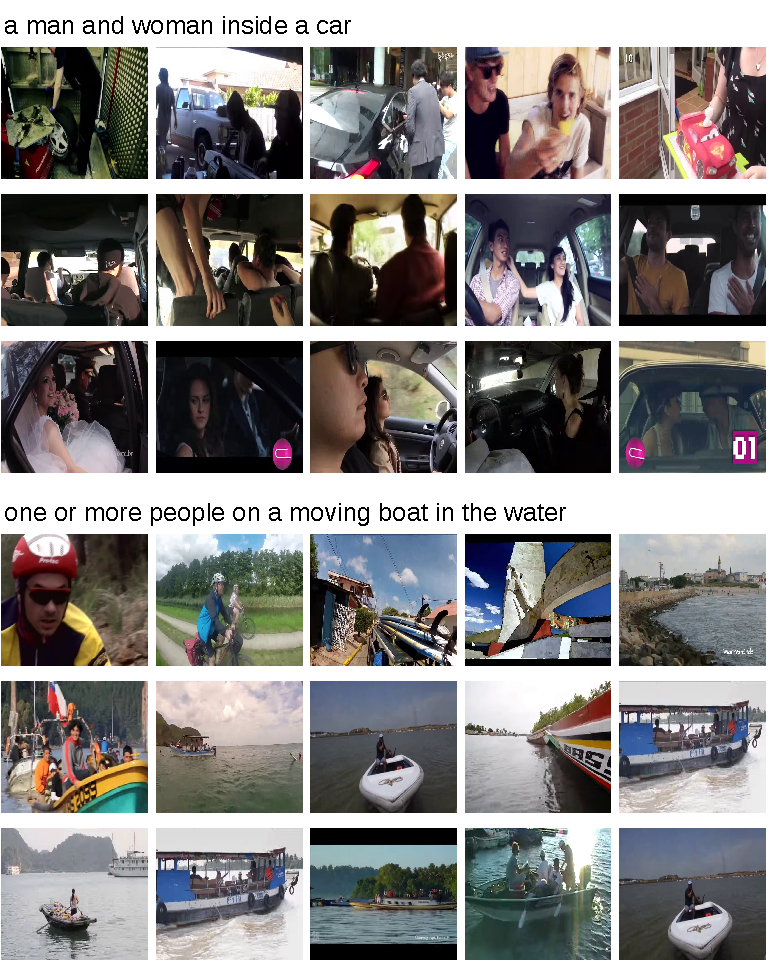
\includegraphics[width=\linewidth]{figures/search_examples2}
    \caption[即席视频检索结果展示(续)]{\textbf{即席视频检索结果展示(续)。对于来自TRECVID AVS评测~\cite{awad2016trecvid,awad2017trecvid,awad2018trecvid,awad2019trecvid}的查询句子,从超过一百万个未标注的视频的大规模的视频集V3C1~\cite{berns2019v3c1}中检索出与查询最相关的前5个视频。对于每个查询,第一行、第二行、第三行分别显示的是W2VV、W2VV++和SEA模型的检索结果。为了更好地展示检索效果,这里展示的是视频的关键帧。}}
    \label{fig:search_examples2}
\end{figure*}


\section{本章小结}
在本章,我们详细地在两个公开的数据集MSR-VTT~\cite{msrvtt}和TRECVID AVS任务数据集~\cite{awad2016trecvid}上评测了在本文提出的W2VV++算法模型和SEA算法模型的有效性。本文提出的W2VV++算法在原来的W2VV算法~\cite{dong2018predicting}的基础上进行了改进,即使用了ITRL目标函数替换原来的MSE函数,使用GRU编码器输出的所有隐藏层状态的平均,而不仅是使用GRU编码器最后时刻的输出状态,通过消融实验证明了这两个改进在即席视频检索上都是有效的,而使用ITRL目标函数提高的效果最明显。本文提出的的SEA算法在W2VV++的基础上使用多空间多目标函数的方式融合多个文本编码器,通过消融实验验证了这种多空间多目标函数的方式可以非常有效地融合不同的文本编码器。通过与目前在视频检索上先进的算法进行对比,证明了W2VV++算法和SEA算法具有很大的优越性,其中单模型的SEA在TRECVID上进行评测的通过多个模型后融合的方法取得的结果,这在即席视频检索上是一个很大的进步。

